\documentclass[tikz,border=6pt]{standalone}
\usepackage{amsmath,amssymb}
\usetikzlibrary{calc,arrows.meta}
\newcommand{\seg}[2]{\overline{#1#2}}

\begin{document}
	
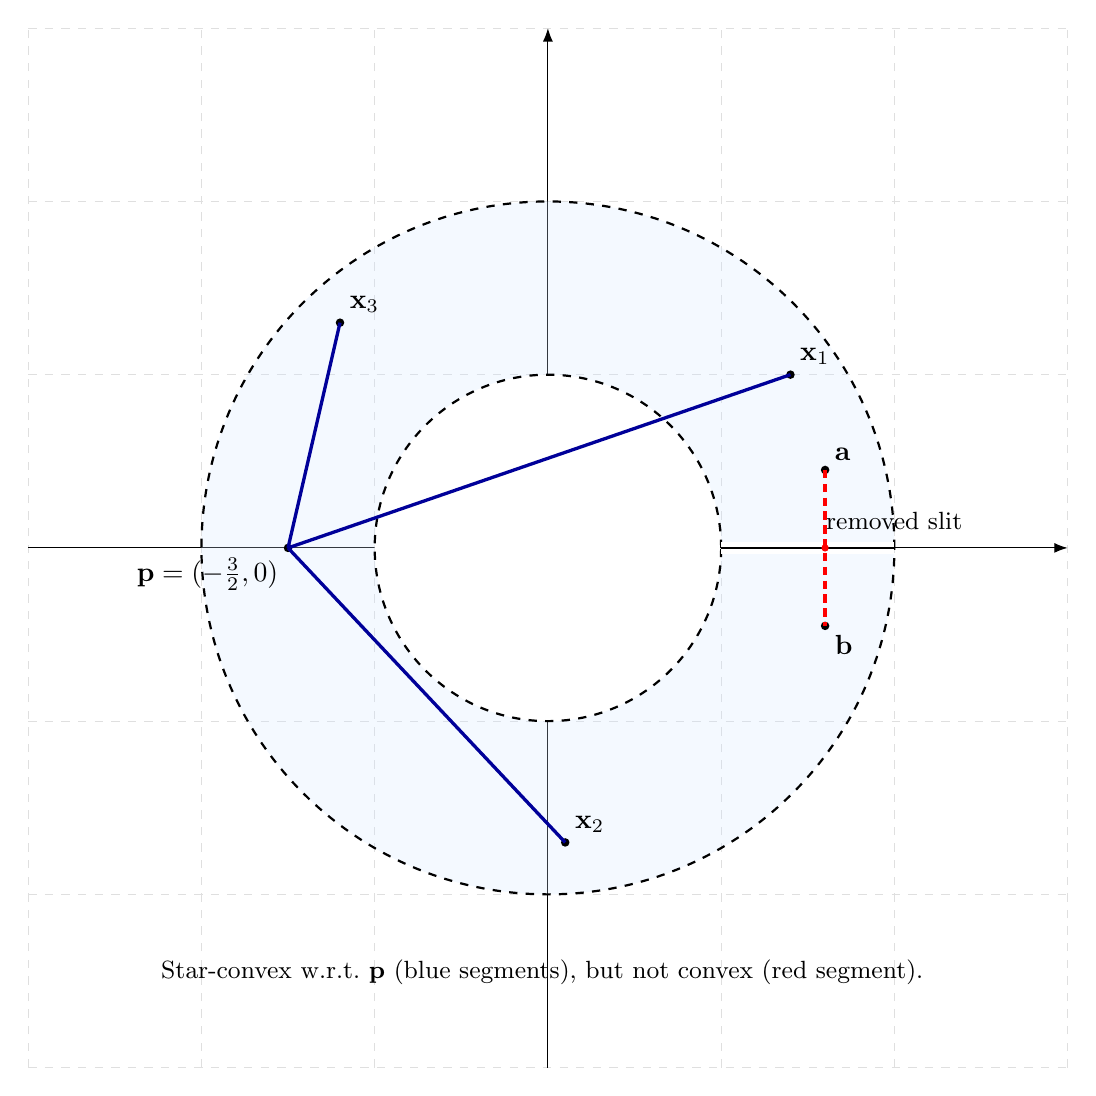
\begin{tikzpicture}[scale=2.2,>=Latex]

\draw[gray!25, dashed] (-3,-3) grid (3,3);
\draw[->] (-3,0) -- (3,0);
\draw[->] (0,-3) -- (0,3);

% Radii
\def\rinner{1.0}
\def\router{2.0}

% Fill annulus
\definecolor{region}{RGB}{210,230,255}
\fill[region, opacity=.25] (0,0) circle (\router);
\fill[white] (0,0) circle (\rinner);

% Boundaries (dashed to suggest openness)
\draw[dashed,thick] (0,0) circle (\router);
\draw[dashed,thick] (0,0) circle (\rinner);

% Removed slit along positive x-axis
\draw[line width=4.2pt,white] (\rinner,0) -- (\router,0);
\draw[thick] (\rinner,0) -- (\router,0);
\node[above right] at (1.55,0.05) {\small removed slit};

% Star center p
\coordinate (p) at (-1.5,0);
\fill (p) circle (0.7pt);
\node[below left] at (p) {$\mathbf{p}=(-\tfrac32,0)$};

% Sample points x_i and segments to p
\coordinate (x1) at (1.4,1.0);
\coordinate (x2) at (0.1,-1.7);
\coordinate (x3) at (-1.2,1.3);

\foreach \X/\lab in {x1/\mathbf{x}_1,x2/\mathbf{x}_2,x3/\mathbf{x}_3}{
	\fill (\X) circle (0.7pt);
	\node[above right] at (\X) {$\lab$};
	\draw[very thick,blue!60!black] (p) -- (\X);
}

% Non-convexity points a,b with segment crossing slit
\coordinate (a) at (1.6,0.45);
\coordinate (b) at (1.6,-0.45);
\fill (a) circle (0.7pt);
\fill (b) circle (0.7pt);
\node[above right] at (a) {$\mathbf{a}$};
\node[below right] at (b) {$\mathbf{b}$};

\draw[very thick,red,densely dashed] (a) -- (b);
\fill[red] (1.6,0) circle (0.6pt);
%\node[red,align=left] at (2.vex};05,0.0) {\small $\seg{\mathbf{a}}{\mathbf{b}}$ meets the slit\\[-1pt]\small hence not con

% Caption
\node[align=center] at (0,-2.45) {\small
	Star-convex w.r.t.\ $\mathbf{p}$ (blue segments), but not convex (red segment).
};
\end{tikzpicture}	
	
%	% ============================================================
%	% Figure 1: Star-convex but not convex (annulus with a slit)
%	% U := {1<r<2} \ { (x,0): 1<x<2 } in R^2, star-center p = (-3/2,0).
%	% ============================================================
%	\begin{tikzpicture}[scale=2.2,>=Latex]
%		
%		% Parameters
%		\def\rinner{1.0}
%		\def\router{2.0}
%		
%		% Colors
%		\definecolor{region}{RGB}{210,230,255}
%		
%		% --- Draw the annulus region (as a filled ring) ---
%		% Fill outer disk
%		\fill[region] (0,0) circle (\router);
%		% Punch inner disk (white)
%		\fill[white] (0,0) circle (\rinner);
%		
%		% --- Draw boundaries (dashed to suggest openness) ---
%		\draw[dashed,thick] (0,0) circle (\router);
%		\draw[dashed,thick] (0,0) circle (\rinner);
%		
%		% --- Draw the removed slit along the positive x-axis, from r=1 to r=2 ---
%		% Use a thick white line to "cut" the region, then outline it.
%		\draw[line width=4.2pt,white] (\rinner,0) -- (\router,0);
%		\draw[thick] (\rinner,0) -- (\router,0);
%		
%		% --- Star center p ---
%		\coordinate (p) at (-1.5,0);
%		\fill (p) circle (0.7pt);
%		\node[below left] at (p) {$\mathbf{p}$};
%		
%		% --- Some sample points x_i in U and segments to p ---
%		\coordinate (x1) at (1.4,1.0);
%		\coordinate (x2) at (0.1,-1.7);
%		\coordinate (x3) at (-1.2,1.3);
%		
%		\foreach \X/\lab in {x1/\mathbf{x}_1,x2/\mathbf{x}_2,x3/\mathbf{x}_3}{
%			\fill (\X) circle (0.7pt);
%			\node[above right] at (\X) {$\lab$};
%			\draw[very thick,blue!60!black] (p) -- (\X);
%		}
%		
%		% --- Show non-convexity: choose two points whose segment crosses the removed slit ---
%		\coordinate (a) at (1.6,0.45);
%		\coordinate (b) at (1.6,-0.45);
%		\fill (a) circle (0.7pt);
%		\fill (b) circle (0.7pt);
%		\node[above right] at (a) {$\mathbf{a}$};
%		\node[below right] at (b) {$\mathbf{b}$};
%		
%		% Segment a--b crosses the slit, hence not contained in U
%		\draw[very thick,red,densely dashed] (a) -- (b);
%		\node[red] at (2.15,0) {\small segment $\overline{\mathbf{a}\mathbf{b}}$ crosses the slit};
%		
%		% --- Annotation title ---
%		\node[align=center] at (0,-2.45) {\Large
%			\(\displaystyle U=\{1<\|\mathbf{x}\|<2\}\setminus\{(x,0):1<x<2\}\)\\
%			\small Star-convex w.r.t. \(\mathbf{p}\), but not convex
%		};
%		
%	\end{tikzpicture}
%	
%	\vspace{1.2cm}
%	
%	% ============================================================
%	% Figure 2: Not star-convex (punctured plane)
%	% V := R^2 \ {0}; for any p != 0, choose x = -p, segment hits 0.
%	% ============================================================
%	\begin{tikzpicture}[scale=2.2,>=Latex]
%		
%		% Draw a "view window" as a square, to represent (part of) R^2
%		\draw[thick] (-2.2,-2.2) rectangle (2.2,2.2);
%		\node[above] at (0,2.2) {\small (window showing \(V=\mathbb{R}^2\setminus\{0\}\))};
%		
%		% Mark the removed point (the puncture) at the origin
%		\coordinate (O) at (0,0);
%		\draw[thick] (O) circle (0.10);
%		\node[below left] at (O) {$0$};
%		
%		% Pick p and x = -p
%		\coordinate (p2) at (1.4,0.9);
%		\coordinate (x2) at (-1.4,-0.9);
%		
%		\fill (p2) circle (0.7pt);
%		\fill (x2) circle (0.7pt);
%		\node[above right] at (p2) {$\mathbf{p}$};
%		\node[below left] at (x2) {$\mathbf{x}=-\mathbf{p}$};
%		
%		% Segment from p to x; it passes through 0
%		\draw[very thick,red] (p2) -- (x2);
%		
%		% Emphasize the intersection at the puncture
%		\fill[red] (O) circle (0.6pt);
%		\node[red,align=left] at (1.15,-0.15) {\small
%			\(\overline{\mathbf{p}\mathbf{x}}\) meets \(0\notin V\)\\
%			\small so \(V\) is not star-convex};
%		
%	\end{tikzpicture}
	
\end{document}
